\documentclass{llncs}
\pdfpagewidth=8.5truein
\pdfpageheight=11truein
\usepackage{llncsdoc}                                          
\usepackage{graphicx}
\usepackage{color}
\usepackage{subfigure}
\usepackage{url}
\usepackage{amsmath}
\usepackage{comment}
\usepackage{cite}

\begin{document}
\title{Robust Monte Carlo Control Policies to Maneuver Tensegrity Robots out of Obstacles}

\author{Steven Lessard\inst{1} \email{slessard@ucsc.edu}
\and Jonathan Bruce\inst{1} \email{jebruce@ucsc.edu}
\and Adrian Agogino\inst{2} \email{adrian.k.agogino@nasa.gov}
\and Vytas SunSpiral\inst{3} \email{vytas.sunspiral@nasa.gov}
\and Mircea Teodorescu\inst{1} \email{mteodore@ucsc.edu}}
\institute{University of California, Santa Cruz \and UC Santa Cruz, University Affiliated Research Center (at NASA Ames) \and Stinger Ghaffarian Technologies}
%\alignauthor Steven Lessard\\%\titlenote{Main Author and contributor to this work.}\\
%       \affaddr{UC Santa Cruz}\\
%       \affaddr{1156 High Street}\\
%       \affaddr{Santa Cruz, CA 95064, USA}\\
%       \email{slessard@ucsc.edu}
% 2nd. author
%\alignauthor Jonathan Bruce\\%\titlenote{Cheif Editor of LaTeX.}\\
%       \affaddr{UC Santa Cruz}\\
%       \affaddr{1156 High Street}\\
%       \affaddr{Santa Cruz, CA 95064, USA}\\
%       \email{jebruce@ucsc.edu}
% 3rd. author
%\alignauthor Adrian Agogino\\%\titlenote{This was the main advisor for the machine learning.}\\
%       \affaddr{UC Santa Cuz / NASA Ames}\\
%       \affaddr{MS 269-3}\\
%       \affaddr{Moffett Field, CA 94035, USA}\\
%       \email{adrian.k.agogino@nasa.gov}
%\and  % use '\and' if you need 'another row' of author names
% 4th. author
%\alignauthor Vytas SunSpiral\\
%       \affaddr{SGT Inc. / NASA Ames}\\
%       \affaddr{MS 269-3}\\
%       \affaddr{Moffett Field, CA 94035, USA}\\
%       \email{vytas.sunspiral@nasa.gov}
% 5th. author
%\alignauthor Mircea Teodorescu\\
%       \affaddr{UC Santa Cruz}\\
%       \affaddr{1156 High Street}\\
%       \affaddr{Santa Cruz, CA 95064, USA}\\
%       \email{mteodore@ucsc.edu}

\maketitle

%\centerline{AAMAS Paper 75}

\begin{abstract}
{ 
    Multiagent learning has been shown to be effective in creating control policies for sophisticated soft-robotic systems based on tensegrity structures (built from interconnected rods and cables). 
The distributed nature of the tension network within a tensegrity structure along with its smooth distribution of forces is a natural match for distributed learning. 
Indeed, multiagent learning has been used to make control policies that allow tensegrity robots to roll efficiently, climb hills and even go over obstacles. 
In this paper, we extend these results allowing a tensegrity robot to take advantage of its flexible structure to escape deep trenches, a situation that is usually unrecoverable regarding traditional rovers. 
%Ideally, we would like to extend these results to allow a tensegrity robot to take advantage of its flexible structure to escape deep trenches, a situation that is usually unrecoverable regarding traditional rovers. 
Usually these problems are tightly coupled with large, flat search spaces which are difficult for typical multiagent learning. 
%Unfortunately solutions to these difficult problems are often tightly coupled with a "needle in haystack" like search space, making it difficult for multiagent learning. 
As an alternative, we show how a two-step Monte Carlo algorithm combined with a simplified control space based on sinusoid actuations can be used to solve this problem. 
Using this technique, we are able to create control policies that allows a ball-shaped tensegrity robot to escape craters. 
To further investigate the utility of these control policies on these flexible structures, we were able to implemented this technique on under-actuated versions of our tensegrity robot model.
%To further investigate the utility of these control policies, we have also tested the ability of structure to escape using only some of its actuators.
We found that although a decrease in the number of functioning actuators made it more difficult for the robot to escape a crater, some control policies still allowed the robot to successfully escape, despite this limitation.
This success is an important step in creating a robot that can navigate reliably over difficult terrains.
    }
\end{abstract}

\section{Introduction}
\label{introduction}

In this paper, a technique is proposed which enables an extraterrestrial rover based on a tensegrity structure to escape from craters or ditches.
In a real planetary exploration mission, extremely careful planning is taken to insure a rover never moves over a small crater or crevice.
This careful planning can hinder the rover from exploring interesting science near an area with these difficult terrain profiles.
Tensegrity rovers have already been shown to do an excellent job performing scientific tasks in tough places and positions \cite{iscen2013robust}, so finding an optimal controller for these rovers can enable the use of these robots as a scientific agents extraterrestrially.

Tensegrity structures are passively compliant structures which are composed of compression elements suspended within a network of tension elements, as seen in figure \ref{NTRT_sb_example}.
\begin{figure}
\centering
{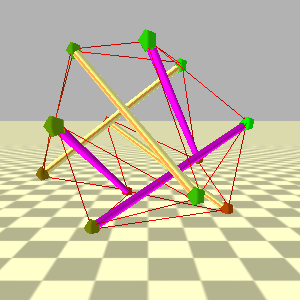
\includegraphics[width=0.9\linewidth]{Pictures/6strut.png}} 
\caption{A simulated tensegrity structure built within NTRT. 
Each of the six rods is 1.5 meters long to model tensegrity structures currently being researched at the NASA Ames Research Center.}
\label{NTRT_sb_example}
\end{figure}
These structures feature a flexible design that counteracts the shortcomings of current surface exploration rovers.
They are impact resistant and lightweight structures that ideally have no bending or shear forces that must be resisted.
They also globally distribute forces to all members, decreasing the magnitude forces induced into a single element.
%A tensegrity robot is therefore a robotic platform based upon the tensegrity structure.
Control of tensegrity structures is still a very open question, with progress made by \cite{Iscen2013a, Tietz2013, mirletz2014design, Caluwaerts2013rsif, GraellsRovira2009, du2014dynamic} for basic mobility even over complex and rough terrain.
Though, the control law for basic mobility may not be enough to enable the rover out of certain terrains.
This paper focuses on a previously unexplored area of robotic maneuvers, escaping a deep trench or craters.

Current planetary and lunar rovers are constrained by traditional robotic attirubutes. 
The wheels found on these rovers only allow the robot to locomote on relatively smooth and level surfaces. 
In addition, non-structurally compliant parts prevent large impact forces on the robot and generate single-points-of-failure.
Due to their fragility, these robots require expensive measures must be taken to ensure protection during transportation, landing, and locomotion.

Tensegrity robots, however, feature a flexible design that counteracts the shortcomings of current rovers.
Their composition of rods and cables creates a impact resistant skeleton, removing the need for costly cushioning during transportation and landing.
This in turn allows for an increase in the proportion of scientific equipment to payload per mission trip.
Inherent redundancy in design means that the failure of a single cable or rod will not jeopardize the viability of the tensegrity rover.
Previously explored punctuated-rolling locomotion in tensegrity rovers has shown that these robots are capable of navigating rough terrain that traditional rovers cannot maneuver\cite{Iscen2013a}. 
Neither current rovers nor traditional rovers have a method for escaping particularly treacherous ground.

Additionally, tensegrity structures possess an ability that allows them to function even when some of their cables can no longer actuate.
This redundancy protects tensegrity robots from single points of failure, an attribute which traditional rovers lack.
By simulating situations in which tensegrity rovers cannot actively use all of their cables, work around solutions can be developed on-the-fly.
This is particularly useful if during an extraterrestrial mission, unexpected mechanical errors inhibit the capabilities of the rover (e.g a motor failure or a broken cable).

Our proposed solution to this is a learning module that teaches tensegrity rovers how to escape ditches and craters on-the-fly.
Our solution consists of two tiers of sampling simulations according to their control policies.

In a given environment, a tensegrity can optimize its existing control algorithm to match the scenario with which it is faced.
This allows for on-board path planning to escape whatever physical obstacles is blocking the movement of the robot.

\section{Implementation}
\label{implementSection}
Our proposed solution is a learning module that teaches a tensegrity rover how to escape trenches and craters.
Given the environment and an existing control algorithm for movement, the tensegrity rover can optimize its movements to match the scenario. 
This allows for on-board path planning to escape trenches, craters, or other physical barriers blocking the rover's movements.

The NASA Tensegrity Robotics Toolkit (NTRT) is a pivotal simulator for exploring the complex dynamics of tensegrity robots. 
NTRT is built on the Bullet Physics Engine, version 2.82, and is an open source platform for the design and control of tensegrity structures and robots\footnote{Additional information about NTRT can be found at \\ \url{http://irg.arc.nasa.gov/tensegrity/NTRT}}.
In order to create structures within the toolkit, a set of builder tools are utilized which specify geometric rods and connecting cables as a set of Cartesian coordinates.
These structures can then be specified as substructures and manipulated in three dimensional space as necessary to build complex tensegrity structures.

%- brief description of the "bullet engine" \\
%    - see 4.1 of "Tensegrity Based Probes"
%- What are the advantages of this approach? What would somebody need to run it etc. Please make reference to as many papers as you can that make a very good case for this approach.

The tensegrity structure used in this paper is a 6-rod icosahedron with 24 actuating cables, each of which is called a muscle. 
This structure was chosen to mimic the Dynamic Tensegrity Robotics Lab's research at the NASA Ames Research Center into exploring tensegrities as an option for extraterrestrial rovers \cite{NIACfinalreport, bruce2014design, sabelhaus2014hardware}.
For the muscle model, a linear spring model consisting of two points implementing Hooke's law with a linear damping term is used as defined in \eqref{hooke}.

\begin{align}
F = -kX - bV \label{hooke}
\end{align}

A simple change in length motor model is also implemented within each muscle, where the muscle is deformed by changing the rest length of the spring model.

% TODO: Line below, rewrite
%In a standard icosahedron where all cable lengths are the same has 8 equilateral triangle faces.
%

\subsection{Controller Definition}
\label{controllerdefn} {
It has been shown by Kim et al in \cite{kim2014rapid} that controlled locomotion may be achieved by deforming only the equilateral, triangular faces on a tensegrity structure.
By consulting the results in \cite{kim2014rapid}, we not only ensured locomotion in the robot, but we were also able to reduce our search space by segregating the muscles according to the equilateral faces.
Each cluster is a set of three muscles conjoined to form one of the $8$ equilateral triangular faces.
To actuate our tensegrity structure, a control algorithm was created to generate synchronized motion between these clusters.

A complex approach, based on this method towards locomotion, has been used to produce a rolling motion in $6$-rod tensegrities as illustrated by Atil Iscen et al in \cite{iscen2013controlling}.
To further reduce the solution space for our multi-level Monte Carlo simulation, we simplified Iscen's controller such that all actuation in the structure was determined by $8$ sine functions, one for each cluster of muscles.
Each muscle actuates towards a shared goal length within its cluster, but this goal length varies by cluster.
The exact goal length at any time step in the simulation is dictated by a sine wave.
Specifically, our goal muscle lengths are regulated by four sine wave parameters: amplitude, angular frequency, phase change, and DC offset.
The equation defined by these four parameters is shown in equation \eqref{sine}.
\begin{align}
y = Asin(\omega t + \varphi) + D
\label{sine}
\end{align}
Where $A$ is amplitude, $\omega$ is angular frequency, $\varphi$ is phase change, and $D$ is the DC offset.

The amplitude is the maximum deviance from the initial pretension in length to which a muscle can actuate.
The angular frequency is how often a muscle cycles between its maximum length and its minimum length. 
Lower angular frequencies are due to greater acceleration by the motor.
The phase change is the length of a muscle at the start of the simulation (i.e. at which point during its period the sine wave begins).
The DC offset is the default length of a muscle.
These four sine wave parameters together dictate the resulting goal length of a muscle.
Each controller, therefore, requires $32$ input parameters to function (the $4$ sine wave parameters for $8$ different clusters).

The control policy of the tensgrity structure is dictated by these $32$ sine wave parameters.
Each simulation run in our experiment has a unique control policy.
The $32$ values in a given control policy are Monte Carlo values within the range of $[0,1]$.
These values are then scaled according to their corresponding sine wave parameter. 
The result is that the control policy, the $32$ sine wave parameters, commands all of the motion generated by our tensegrity structure.
}
  
\subsection{Control Parameter Constraints}
\label{sineconstraints} {
Each sine wave parameter was constrained to real-world limitations.
Since actuators outside of simulation can only ever stretch as far as their material properties allow, the amplitudes in simulation follow this physical constraint.
DC offsets less than the minimum length of an actuator are nonsensical, so this sine parameter was limited to the rest length of each muscle.
Likewise, angular frequency was limited to mimic the acceleration limitations of mechanical actuators. 
For this experiment, we limited our amplitudes to be less than fifty percent of the initial length and actuations to occur at frequencies between $0.3$ and $20$ Hz.
The phase change of any sine wave was limited to be within $[-\pi, \pi]$.
The amalgamation of these constraints formed a more accurate model for simulating the tensegrity robot, providing us with more useful results. 
}
\label{robustconstraints} {
To test for actuator robustness and redundancy, we simply limited which cables were able to change length during the simulation.
We can artificially select cables to ``fail'', that is, to never change from their original length.
The cables are still present in the structure, but due to their imposed inability to move, become passive components to the robot as a whole.
For our experiments, we compared structures with $100\%$ of their $24$ actuators still functioning to structures with $75\%$ ($18$) of the cables functioning, and to structures with only $50\%$ ($12$) of the actuators changing with respect to their sine wave control policies.
This comparison illustrates whether or not the reduction of capable actuators in the tensegrity structure dooms the entire robot.
}
                                                                                                                                   
\subsection{Simulation Execution}
\label{simexec} {
To simulate a tensegrity structure becoming trapped in a crevice, four walls were created to enclose the robot. 
As seen in Figure \ref{escapemontage}, the robot was placed in the middle of these four walls such that the only way it could escape was by climbing out over an edge of the crevice. 
Once the robot had completely removed itself, it simply falls off the wall.
This not only prevented the robot from accidentally re-entering the crater, but prevented the robot from returning within $25$ meters of its origin (the center of the crater).
As a result, recorded displacements of over $25$ meters indicate a successful escape.

\begin{figure}
\centering
\subfigure[$t_0$]{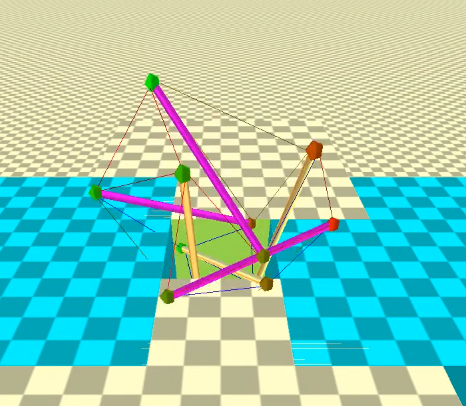
\includegraphics[height=0.49\linewidth, width=0.49\linewidth]{Pictures/Escape_1.png}} 
\subfigure[$t_0+0.5s$]{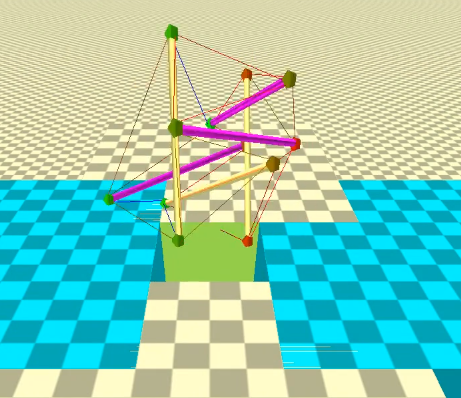
\includegraphics[height=0.49\linewidth, width=0.49\linewidth]{Pictures/Escape_2.png}} 
\subfigure[$t_0+1.0s$]{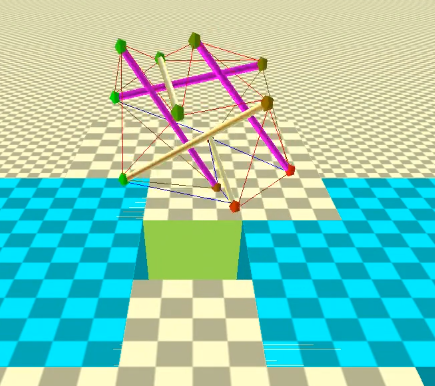
\includegraphics[height=0.49\linewidth, width=0.49\linewidth]{Pictures/Escape_3.png}} 
\subfigure[$t_0+1.5s$]{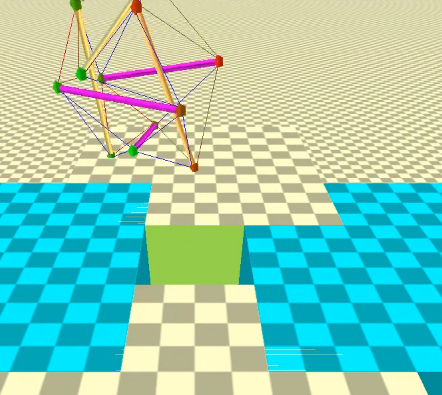
\includegraphics[height=0.49\linewidth, width=0.49\linewidth]{Pictures/Escape_4.png}} 

%\subfigure[$\eta=0.1$]{\includegraphics[width=0.45\linewidth]{pressure_curves_etapoint1_h1h2point1.pdf}}\\
%\subfigure[$\eta=0.2$]{\includegraphics[width=0.45\linewidth]{pressure_curves_etapoint2_h1h2point1.pdf}}
\caption{A tensegrity structure escaping a crater. 
The crater has roughly a 25m radius at its closest edge and is elevated above the ground to keep the escaped tensegrity robots out.
}
\label{escapemontage}
\end{figure} 

To test our controllers in the simulator, we established a two-tier system for sampling control policies.
We define a sample as a single simulation run and we define a tier as the set of samples that are run according to the same high level policy.
We also define a generation to be an individual tier within a given experiment.
In the first tier of sampling, we set control policies according to a uniform distribution of Monte Carlo values.
Each of these Monte Carlo values correspond to one of the $32$ parameters which dictate the actuations of our robot with respect to time.
By determining which control policies caused the tensegrity robot to escape from its crater, we can segregate samples as either successes (escaped) or failures (not escaped).
The successful samples from the first tier are used to centralize the sampling ranges for the second tier.
In this second tier, the control policies of the simulated robots are made to imitate already-successful control policies.
The only difference in sampling policy for this new tier is that each Monte Carlo value in the second tier is sampled uniformly within an acute range which is centered around ``trustworthy'' Monte Carlo values for that particular parameter.
 
Each of our samples run for $60,000$ steps.
As a result, a total of $100$ seconds are simulated each sample.
To find enough control policies that successfully generate an escape path, at least one thousand samples were executed in each generation.
Once a sample has finished executing, the control policy of that sample as well as the final displacement of the robot are recorded.

To test actuator robustness, we took $100$ samples of the simulated robot at each of the three actuator settings ($100\%, 75\%, and 50\% actuators enabled)$.
Each of these samples were run for $100$ simulated seconds as well.
}

\subsection{Reward System}
\label{rewardsystem} {
In this experiment, the control policy of an individual sample was judged to be either a success or a failure.
This judgement depends on that sample's displacement (the distance traveled by the tensegrity rover from its initial position).
The magnitude of the displacement of a simulated tensegrity robot determined the categorization of that sample's control policy.
Specifically, if a displacement was larger than the distance between the crater's origin and the edge of the crater, that displacement indicates the robot successfully escaped the crater.
As a result, the control policies of samples that resulted in a displacement of $25$ meters or more were deemed successes.
All other control policies were considered failures.
The sine wave values that constituted a successful control policy were saved for the next generation while the others were cast out.
This procedure, in summary, sorts data as either capable of generating viable escape paths or as data that is incapable of generating viable escape paths.
}

\subsection{High Level Policy for Generations}
\label{highlevelpolicy} {
Each sample represents a simulation based on a set of $32$ control values and its resulting performance. 
Each generation is then taking samples from the previous generation to help determine which samples to take. 
In Generation 0, control policies of each sample are uniformly random and are determined by the Monte Carlo method.
The Monte Carlo values ranged from $0$ to $1$ inclusive. 
These values were eventually scaled to match the physical requirements as dictated in sub-section \ref{sineconstraints}.
These assigned sine wave values follow an even distribution such that the probability of any given legal value (i.e. $[0,1]$) being assigned is equal to the probability of any other legal value.
For our experiment, we ran $1000$ samples in Generation 0.robot
When every sample in this base generation has finished executing, the recorded results were parsed.
Once the successful samples have been filtered out, their control policies are stored for use in the next generation.

In Generation 1, control policies of each sample consider the already-proven successful policies of Generation 0.
Control policy values in Generation 1 are centered around the respective input policy values from Generation 0.
To optimize the results from Generation 0, the control policy values for Generation 1 are then tweaked by as much as $0.5\%$.
Each of the successful samples from Generation 0 were re-run in Generation 1 ten times, each with a slight variation.
The purpose of this action is to discover what improvements can be made on already successful control policies.
The exact variation on the Generation 1 control policy values is dictated by the Monte Carlo method.
Once again, the selection distribution of this Monte Carlo sampling is even, so each value within $\pm0.05\%$ of the input Generation 0 sine wave values is equally likely to be chosen.
These modified control policies are then simulated en masse.
For our two-tier experiment, we ran $1100$ samples, ten times the number of successful control policies discovered in Generation 0.
As in the base generation, the recorded results are analyzed and the successful samples are filtered out. \\

To test actuator redundancy, we ran $3$ generations of $100$ samples each.
The first generation was our control group (all $24$ actuators functioned according to their sine wave control policies).
The second generation experienced a forced actuator failure in $25\%$ ($6$) of the $24$ actuators.
These ``failed'' actuators became passive components as the other $18$ actuators behaved normally.
The third and final generation only had half ($12$) of its actuators functioning according to sine wave control policies.
}

\section{Results}
\subsection{Results of Two-Tier Monte Carlo Simulations}
\label{resultsSection} {
We ran experiments on the controller of our tensegrity robot to optimize escape paths out of an arbitrary crater.
To measure the success of each control policy, we record the displacement of the corresponding simulated robot.
This displacement is used as a score for comparison against the displacements of other samples.

In addition to the displacement of the robot, the $32$ Monte Carlo values, the control policy of that sample, that generated said displacement were also recorded.
To escape the simulated obstacle, a displacement of at least $25$ meters was required.
Because of the height at which the robot rested on top of the fissure, once a robot escaped (and consequently reached $25$ meters from its origin), it fell out of the crater.
Consequently, all robots that were able to escape remained outside of the crater for the remainder of that trial.
This means that there were no samples in our simulation where a tensegrity robot escaped a crater only to fall back into that crater.

The scatter plots, Figures \ref{gen0scatter} and 4, feature data points for each control policy.
Since each sample has exactly one control policy, there are $1000$ data points in the scatter plot for Generation 0 and $1100$ data points in the scatter plot for Generation 1.
Each data point represents a $32$-dimensional value, the $32$ sine wave parameter control policy.
                     
\label{resultsgen0} {
\begin{figure}
\label{gen0scatter}
\centering
\subfigure[Generation 0]{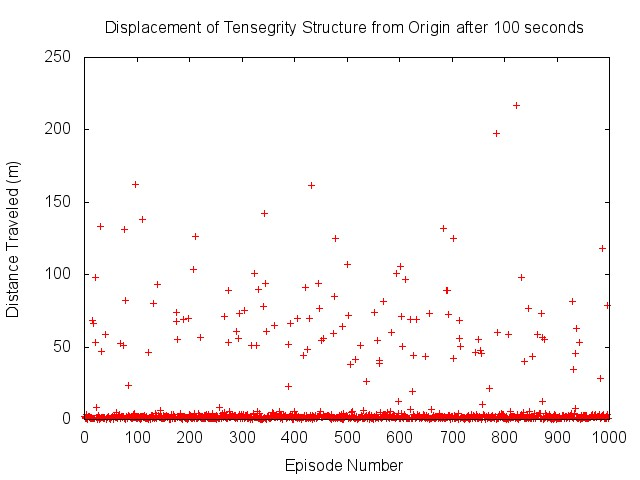
\includegraphics[width=1\linewidth]{Pictures/gen0distances.jpg}} 
\caption{The displacements reached in 1000 independent samples using Monte Carlo generated control policies.}
\end{figure}

%Generation 0 yielded diverse, but uneven results (see Figure \ref{gen0scatter}).
Generation 0 yielded diverse, but uneven results (see Figure $3$).
Displacements ranged from $0.01$ meters to $216.55$ meters.
The mean displacement traveled by the robot was $9.91$ meters and $11.1\%$ of samples resulted in a successful escape.
The vast majority ($88.9\%$) of Generation 0 samples featured a failed control policy (i.e. the robot did not escape the crater).
} 

\label{resultsgen1} {
\begin{figure}
\label{gen1scatter}
\centering
\subfigure[Generation 1]{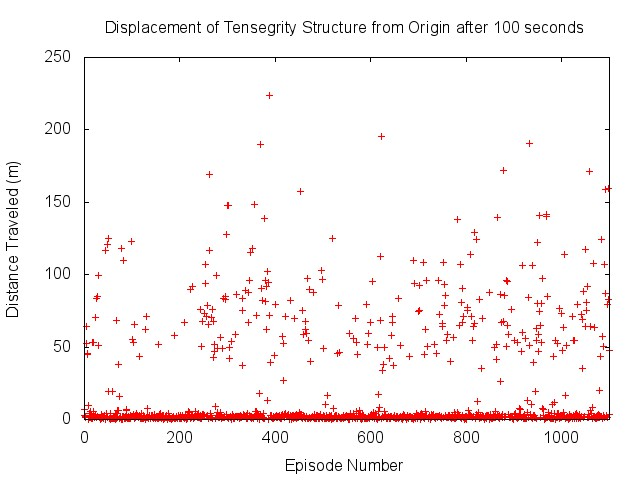
\includegraphics[width=1.0\linewidth]{Pictures/gen1distances.jpg}} 
\caption{The displacements reached in 1100 independent samples using control policies dictated by the successful samples from Generation 0. 
The values in the set of sine wave parameters from Generation 1 samples were each centered around one of the successful corresponding sine wave parameters in Generation 0 control policies.
These Generation 1 values were then modified to be within 0.5\% of their respective Generation 0 values with the goal of optimizing Generation 0 control policies.}
\end{figure}

Generation 1 yielded a larger range of results than Generation 0, most notably including a greater number of successful samples.
Displacements ranged from $0.05$ meters to $223.59$ meters.
The mean displacement traveled by the robot was $20.53$ meters and $24.0\%$ of samples resulted in a successful escape.
The majority ($76.0\%$) of Generation 1 samples featured a failed control policy (i.e. the robot did not escape the crater).
}

\begin{table}
\centering
\caption{Displacement (m) by Generation}
\begin{tabular}{|c|c|c|c|c|} \hline
Generation&Minimum&Average&Maximum&\% Escaped\\ \hline
$0$ & $0.01$ & $9.91$  & $216.55$ & $11.1$\\ \hline
$1$ & $0.05$ & $20.53$ & $223.59$ & $24.0$\\ \hline
\end{tabular}
\end{table}

The combined results from the two high level policies have shown significant improvement from Generation 0 to Generation 1. 
The minimum, average, and maximum displacements in Generation 1 were all improvements over the previous generation.
A randomly selected sample from Generation 1 was $2.16$ times more likely to generate a successful escape path than an arbitrary sample from Generation 0.
The mean displacement of a Generation 1 robot was less than $5$ meters from its goal displacement; a $207\%$ increase from the comparable mean Generation 0 robot.
}

%\section{Discussion}
%\label{discussion} {
%Problem at large, including problem space and reducing said problem space.


 %- a set of figures showing the tensegrity robot moving through the proposed environment \\
%- a table with a series of conditions we are trying to followup \\
%}
                      
\subsection{Results of Actuator Redundancy Experiments}
\label{robust24} {
\begin{figure}
\label{robust24scatter}
\centering
{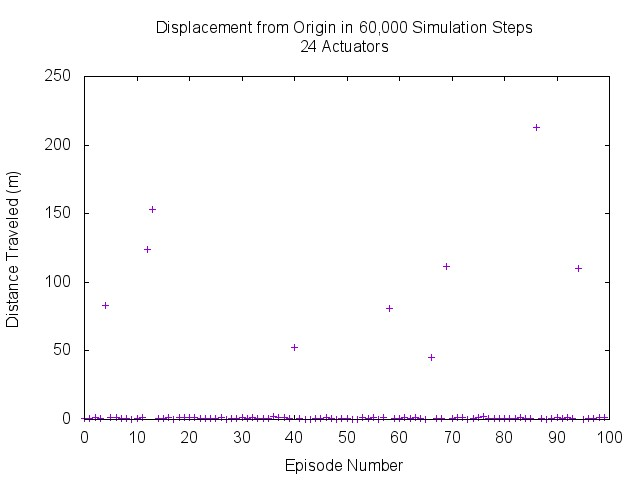
\includegraphics[width=1\linewidth]{Pictures/dists100.jpg}} 
\caption{100 Samples of Tensegrity Structures with 24 Actuators}
\end{figure}

By reducing the number of functioning actuators on our simulated tensegrity, the limitations of tensegrity escape can be better explored.
%With all 24 actuators on the tensegrity functioning correctly, a successful escape is relatively easy ($9\%$ success rate) (see Figure \ref{robust24scatter}).
With all 24 actuators on the tensegrity functioning correctly, a successful escape is relatively easy ($9\%$ success rate) (see Figure $5$).
} 
                       
\label{robust18} {
\begin{figure}
\label{robust18scatter}
\centering
{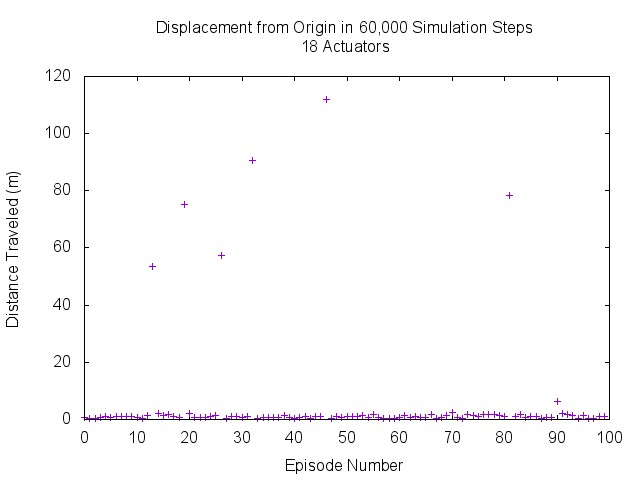
\includegraphics[width=1\linewidth]{Pictures/dists75.jpg}} 
\caption{100 Samples of Tensegrity Structures with 18 Actuators}
\end{figure}

In the second generation, $6\%$ of the tensegrity structures were able to escape.
%With 18 actuators on the tensegrity functioning correctly, a successful escape is more challenging, but not impossible (see Figure \ref{robust18scatter}).
With 18 actuators on the tensegrity functioning correctly, a successful escape is more challenging, but not impossible (see Figure $6$).
} 
                       
\label{robust12} {
\begin{figure}
\label{robust12scatter}
\centering
{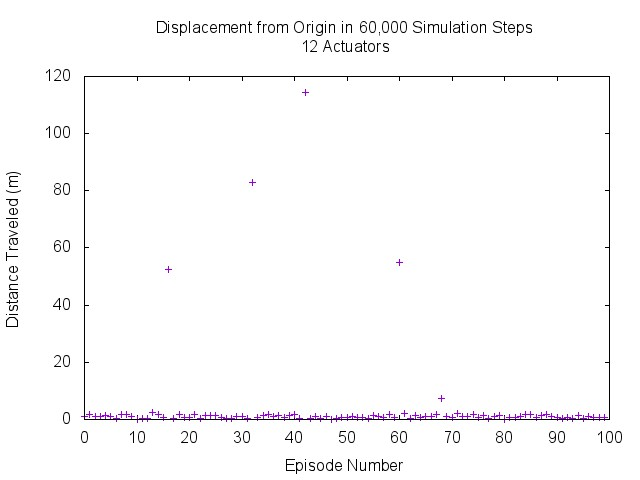
\includegraphics[width=1\linewidth]{Pictures/dists50.jpg}} 
\caption{100 Samples of Tensegrity Structures with 12 Actuators}
\end{figure}

%With just half of the original actuators functioning correctly, a successful escape is even more difficult (see Figure \ref{robust12scatter}).
With just half of the original actuators functioning correctly, a successful escape is even more difficult (see Figure $7$).
In this generation, $4\%$ of tensegrity rovers were still able to escape the ditch in the allotted time.
} 

\label{robustdiscussion} {
These generations of varying actuator capability illustrate a number of important trends.
Our results show that all three generations produced some successful samples.
This indicates that tensegrity robots can still complete the complex task of escaping a crater while performing with a reduced number of actuators.
Since not all actuators were required to escape the crater, the redundancy of tensegrity structures for escaping craters as we have demonstrated is verified.
These results suggest that tensegrity robots will be able to adapt to structural and mechanical malfunctions that might prove fatal to other robots.
More generally, the data suggest that tensegrity robotics as a whole present an inherent benefit for dealing with hazardous situations that threaten the very structure of the robot.
Robots which are most trustworthy can be sent on a larger variety of extraterrestrial missions, exploring environments otherwise inaccessible to traditional rovers.

}
 
\section{Conclusions}
\label{conclusion}
Controlling tensegrity robots is a difficult task due to the novelty of the structures as well as the inherent complexity of actuation patterns.
Unlike most traditional robots, which operate in strictly confined ranges of motion, the flexibility of tensegrity structures allows for a more diverse spectrum of structural configurations.
This complexity, consequently, translates to a plethora of potential control algorithms and classes of controllers.

In order to significantly reduce this overwhelming problem space, we have explored methods to reduce the variation between versions of our controller while retaining a high empirical success rate.
Specifically, our solution intelligently mapped muscles and used very simple control policies (sine waves).
By clustering the muscles in our tensegrity structures into triplets, we reduced our problem space by two thirds.
Sine wave control functions meant that we could completely define the actuator goal length with respect to time of each cluster in only four parameters.
By reducing our problem space, we were able to run Monte Carlo simulations to quickly obtain useful data on escape controllers.

The results from the two generations of simulation have illustrated the compounding improvements that a two-level Monte Carlo simulation can yield.
In Generation 0, uniformly random control policies produced by the Monte Carlo method established a baseline success rate for tensegrity structures escaping our crater.
Generation 1 built off of the information obtained from Generation 0 by sampling around the corresponding values of Generation 0's previously-tested control policies that were shown to succeed.
The result is a proven system that optimizes control parameters for tensegrity robots that must escape craters.

Tensegrity structures, due to their abundance of cables, are able to actuate in a variety of manners.
This redundncy, coupled with the flexibility of the suspended system, allows tensegrit robots to successfully actuate even when limited by ``failed'' actuators.
If our tensegrity rovers lose actuation capability in $6$ or even $12$ of their $24$ actuators, it can still succesfully escape the crater with which it was presented.
This is particularly relevant to the original mission of the rover because loss of mechanical capability is not uncommon in extraterrestrial robots.
This ability to function, even under adverse conditions, can allow for missions to continue when more traditional rovers would fail.
Also, robots with greater redundancy can be trusted to explore more dangerous terrains and environments than their traditional counterparts.
This means scientific data can be recorded from more hazardous missions than previously allowed.

We are currently extending this research in four directions.
First, we are analyzing alternative ways high level policies for Generation 1. 
New high level policies could not only improve benchmarks we have already achieved, but also allow us to explore neighborhoods of successful control policies.
Second, we are investigating the results from generations that use the successful control policies of Generation 1. 
From these future generations, regressions can be determined to formally define the effect of each tier of the Monte Carlo simulations.
Third, we exploring alternatives to the Monte Carlo method for generating control policies in each generation.
A new distribution could accelerate the optimization process and may be necessary if more complex control policies are substituted for our current approach.
Finally, we are further exploring the limitations of actuator redundancy.
By seeing the minimum mechanical requirements for a required motion, a tensegrity rover can determine whether a particular task would be possible during its mission.
This includes analyzing not just how many actuators are needed to function, but which actuators specifically are required, given the orientation and position of the entire system.
We can also explore the failure of cables to not just actuate, but to remain connected at all.
A robot will most likely move differently depending on whether its failed actuators are passive (just failed motors) or completely broken.

\section{Acknowledgments}
This work was partially supported by the NASA Innovative Advanced Technology Program.

\bibliographystyle{splncs03}
\bibliography{TwoTierMonteCarloTensegrity}


\end{document} 
